\documentclass{beamer}
\usepackage[utf8]{inputenc}

% code snippets
% \usepackage{listings}
% \lstset{inputpath=/home/arch/git/2020-docker-talk/content/src}
% \usepackage{minted}
\usepackage{minted}

% biblatex (requires biber; sudo pacman -S biber)
\usepackage[]{biblatex} % biblatex
\addbibresource{"./content/bib/bib1.bib"}
\addbibresource{"./content/bib/bib2.bib"}
\addbibresource{"./content/bib/throwaway.bib"}

\usepackage{graphicx}
\graphicspath{ {./content/img/} }

\usetheme{Boadilla}
\usecolortheme{rose}
\beamerdefaultoverlayspecification{<+->} % this will turn it into slides

\title{Dockerisation}
\subtitle{Container technologies, for ease of development and deployment}
\author{George Onoufriou}
\date{\today}

\begin{document}

  \frame{\titlepage}

  \begin{frame}
    \frametitle{The Problem}
    \begin{itemize}
        \item You write monolithic software (lets say a whole web-stack) on machine A
        \item You test this web-stack on machine A, everything is working fine
        \item You deploy software on machine B (lets say a lab machine), oh no it doesn't have x, y, z installed
        \item You install x, y, z, but on machine A; x was version 1.2, y was version 0.0.1, z was version 1.r23345 so you go through manually install those versions
        \item web-stack still does not work properly as there was an undocumented dependency U, that you never noticed since you were always running on machine A
        \item You break down and question if you know what you are doing, as you struggle to meet a deadline
        \item You pray it works on machine C which it will be evaluated on for an assignment, it doesn't but you proclaim "it worked on my machine"
    \end{itemize}
  \end{frame}

  \begin{frame}
    \frametitle{How This Worked in Industry}
    \begin{figure}[th!]
      \centering
      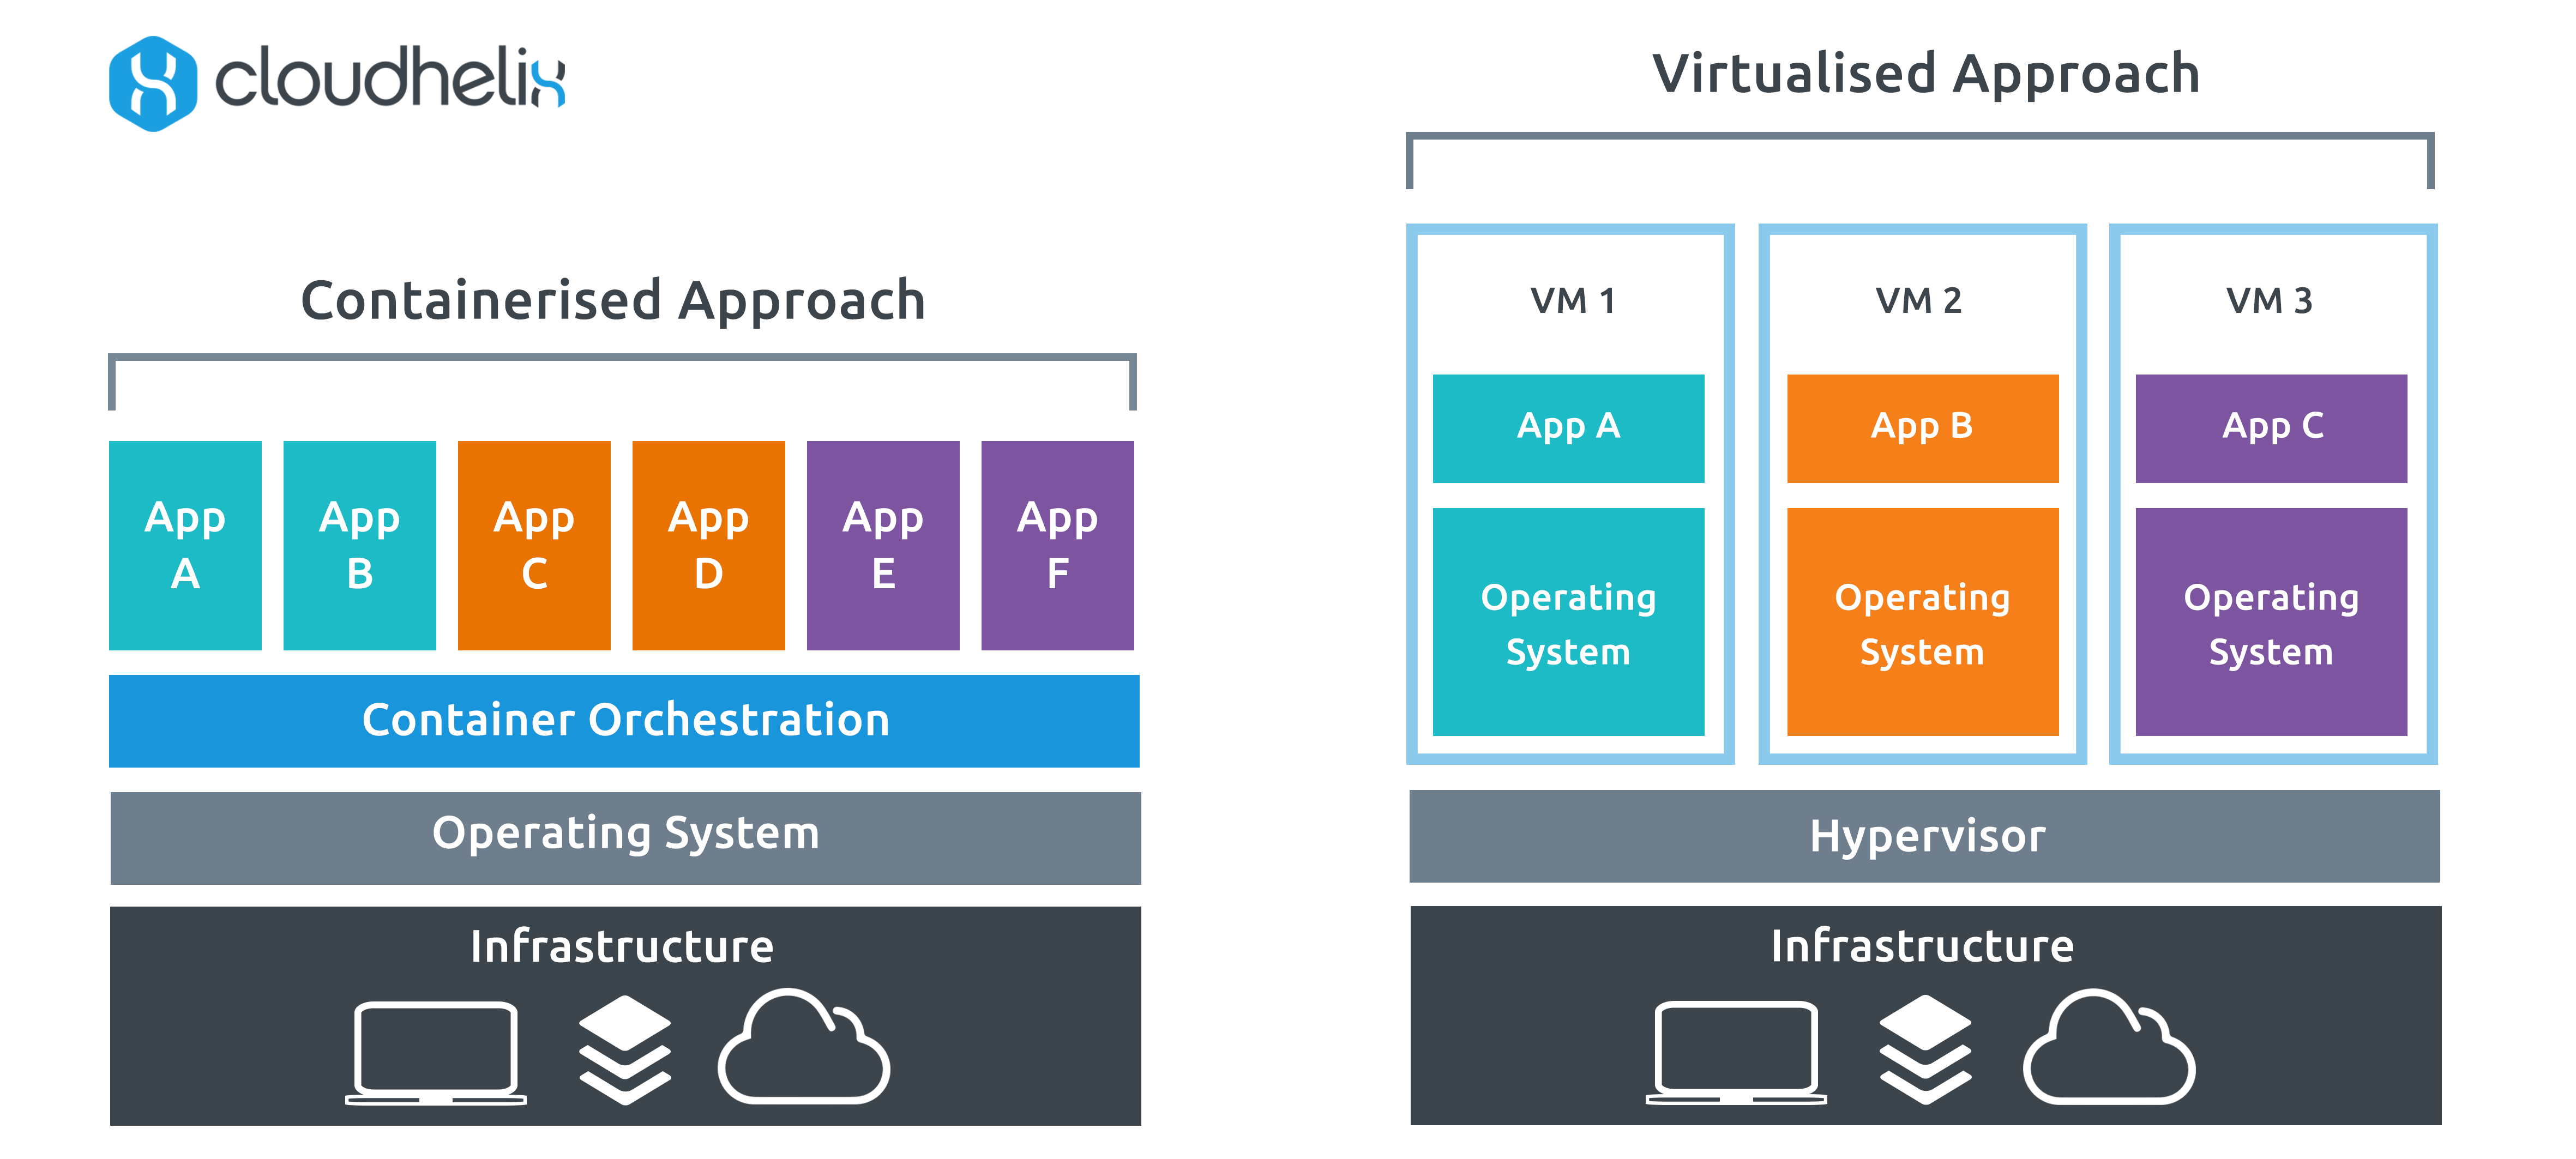
\includegraphics[width=0.9\textwidth]{containerisation.png}
      \caption{Comparing Virtualisation and Containerisation.}
      \label{fig:containerisation}
    \end{figure}
  \end{frame}

  \begin{frame}
    \frametitle{Containerisation Use Cases}
    \begin{figure}[th!]
      \centering
      
\includegraphics[width=0.4\textwidth]{kube_case_studies.png}
      \caption{Sample Kubernetes use in the wild. \autocite{kube_cases}}
      \label{fig:kube_use}
    \end{figure}
  \end{frame}

  \begin{frame}
    \frametitle{What is Docker}
    \begin{itemize}
        \item Repeatable instructions to (re)create a lightweight virtual machine
    \end{itemize}
    \begin{figure}[th!]
      \centering
      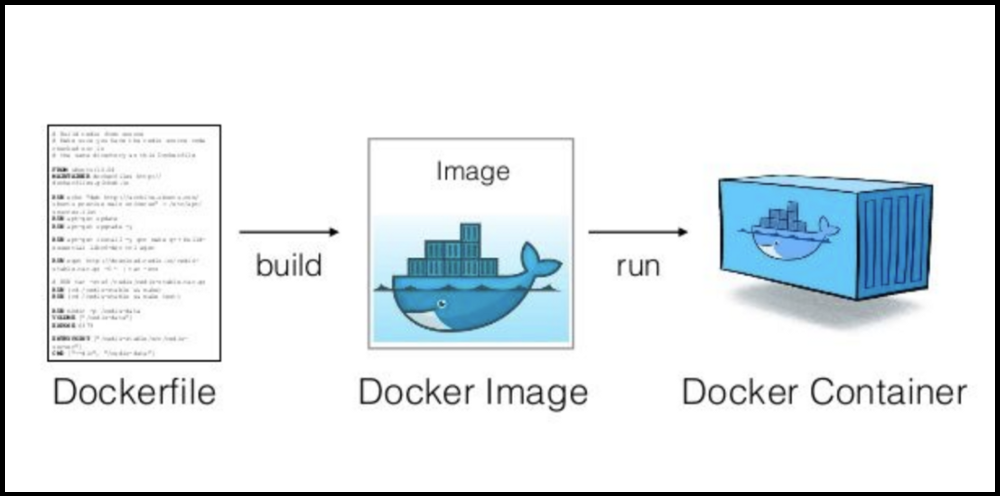
\includegraphics[width=0.7\textwidth]{docker_process.png}
      \caption{Creating Docker Containers. \autocite{docker_build}}
      \label{fig:docker_build}
    \end{figure}
  \end{frame}

  \begin{frame}
    \frametitle{Dockerfile build}
    \inputminted{dockerfile}{content/src/Dockerfile}

  \end{frame}

  \begin{frame}
    \frametitle{Docker Image run}
  \end{frame}

  \begin{frame}
    \frametitle{some frame title}
    Citation \autocite{gentry2009fully, Goodfellow-et-al-2016}
    Image:
    \begin{figure}[th!]
      \centering
      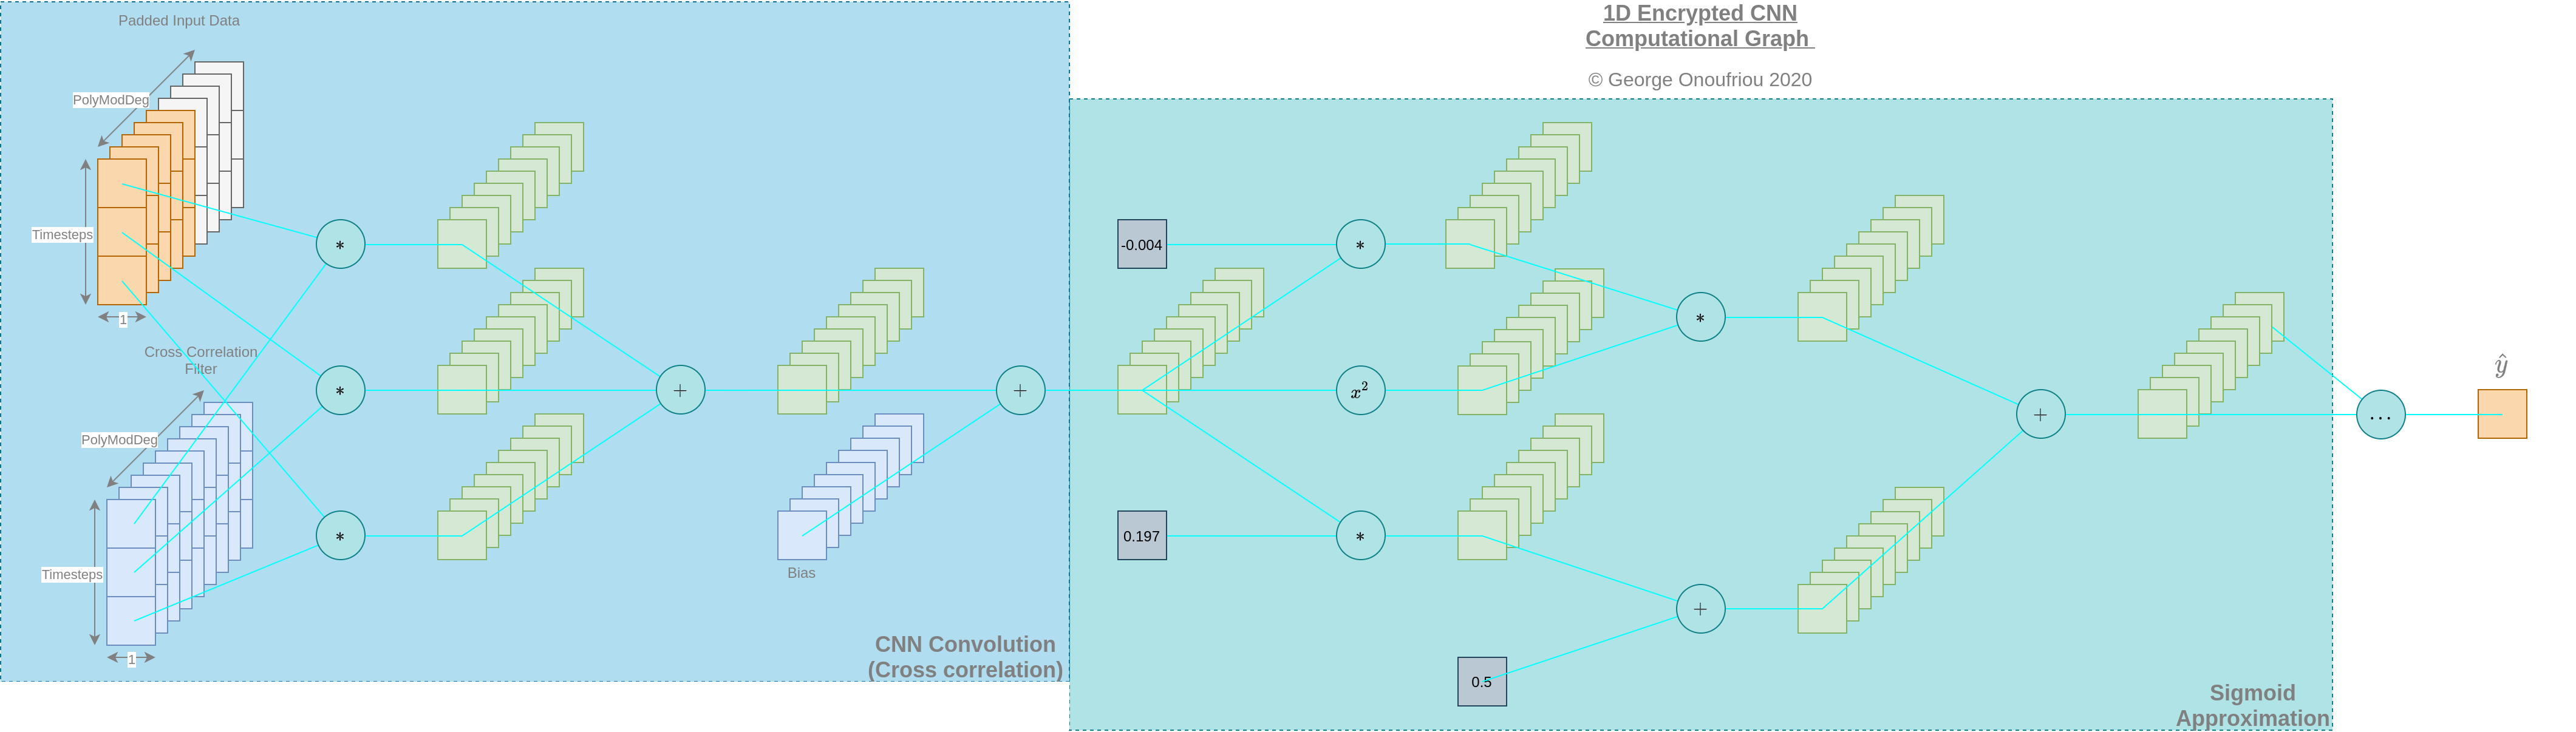
\includegraphics[width=\textwidth]{encrypted_cnn.png}
      \caption{Computational 1D CNN computational graph.}
      \label{fig:gan}
    \end{figure}
  \end{frame}

  \begin{frame}
    \frametitle{equations frame title}
    Equations:
    \begin{equation}
      \label{sigmoid}
      \sigma(x) = \frac{1}{1+e^{-x}}
    \end{equation}
    \begin{equation}
      \label{sigmoid_approx}
      \sigma(x) \approx 0.5 + 0.197x + -0.004x^3
    \end{equation}
    \begin{equation}
      \label{cnn_activation}
      a^{<t>}=\sigma(w_{i}^{<t>}x^{<t>}+b_i^{<t>})
    \end{equation}
    \begin{equation}
      \label{gradient}
      \frac{df}{d\sigma} = (1-\sigma{x}) * \sigma{x}
    \end{equation}
    \begin{equation}
      \label{weight_update}
      % learning rate
      w_i^{j+1<t>} = w_i^{j<t>} - (l * \frac{df}{dw_i^{j<t>}})
    \end{equation}
  \end{frame}

  \begin{frame}[allowframebreaks]
    \frametitle{References}
    % % biblatex version
    \printbibliography
  \end{frame}

\end{document}
